\section{Discretization Methods}

\subsection{Finite Volume Method}
Basically, take a differential equation and integrate it over a control volume. This gives us a discrete form of the equation.
\begin{figure}[H]
    \centering
    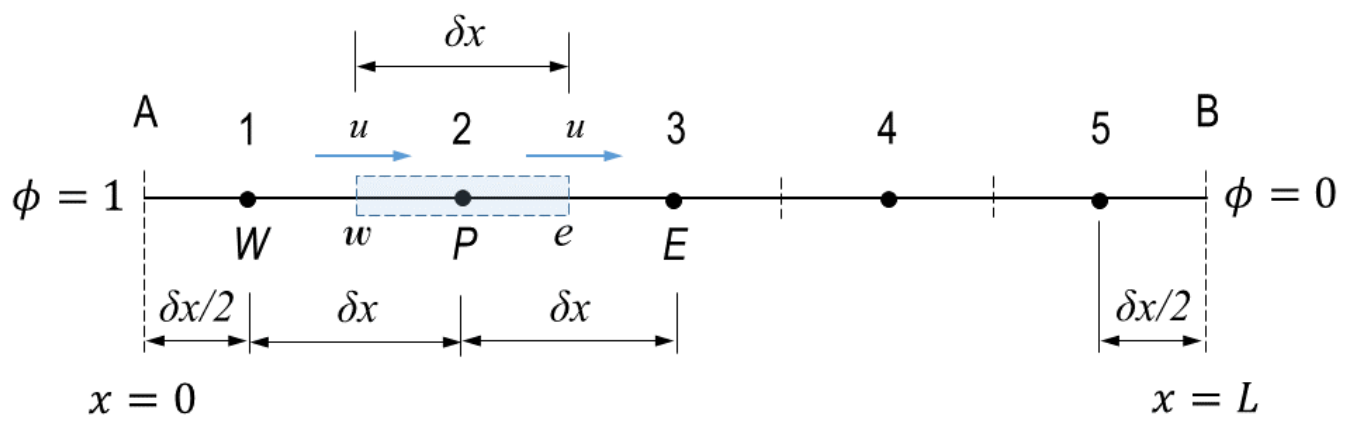
\includegraphics[width=0.8\textwidth]{Section/Figures/mesh generation.png}
    \caption{Grid generation for finite volume method}
\end{figure}
Consider the diffusion-convection equation with no source term:
\begin{align*}
    \frac{d}{dx} (\rho \vec{u} \phi) = \frac{d}{dx} (\Gamma \frac{d\phi}{dx})
\end{align*}
Integrating over the control volume:
\begin{align*}
    \int_{\text{CV}} \frac{d}{dx} (\rho \vec{u} \phi) dV &= \int_{\text{CV}} \frac{d}{dx} (\Gamma \frac{d\phi}{dx}) dV \\
    \int_{\Delta x} \frac{d}{dx} (\rho \vec{u} \phi) S dx &= \int_{\Delta x} \frac{d}{dx} (\Gamma \frac{d\phi}{dx}) S dx \\
    \left[ \rho \vec{u} \phi \right]_{w}^{e} &= \left[ \Gamma \frac{d\phi}{dx} \right]_{w}^{e} \\
    [\rho \vec{u} \phi]_{e} - [\rho \vec{u} \phi]_{w} &= \left[\Gamma \frac{d\phi}{dx} \right]_{e} - \left[\Gamma \frac{d\phi}{dx} \right]_{w} 
\end{align*}

\subsubsection{Central Difference Scheme}
The derivative terms can be approximated using the central difference scheme. 
\begin{empheq}[box=\fbox]{align}
    \frac{d\phi}{dx}_e & = \frac{\phi_E - \phi_P}{\Delta x_{PE}} \\
    \frac{d\phi}{dx}_w & = \frac{\phi_P - \phi_W}{\Delta x_{WP}}
\end{empheq}
For $\phi$ at the non-node points, the central difference scheme calculates the values of $\phi$ at $e$ and $w$ using linear interpolation:
\begin{empheq}[box=\fbox]{align}
    \phi_e & = \frac{\phi_P + \phi_E}{2} \\
    \phi_w & = \frac{\phi_P + \phi_W}{2}
\end{empheq}
And at Node 1 ($\phi_{W} = \phi_{A}$),
\begin{empheq}[box=\fbox]{align}
    \frac{d\phi}{dx}_w & = \frac{\phi_P - \phi_A}{\Delta x_{AP}} \\
    \phi_w & = \phi_A
\end{empheq}
And at Node N ($\phi_{E} = \phi_{B}$),
\begin{empheq}[box=\fbox]{align}
    \frac{d\phi}{dx}_e & = \frac{\phi_B - \phi_P}{\Delta x_{PB}} \\
    \phi_e & = \phi_B
\end{empheq}

Substituting these values into the finite volume equation:
\begin{align*}
    \rho \vec{u} \frac{\phi_E - \phi_P}{\Delta x_{PE}} - \rho \vec{u} \frac{\phi_P - \phi_W}{\Delta x_{WP}} &= \Gamma \frac{\phi_E - \phi_P}{\Delta x_{PE}} - \Gamma \frac{\phi_P - \phi_W}{\Delta x_{WP}} 
\end{align*} 
And then you can write it in the form
\begin{align*}
    a_P \phi_P = a_W \phi_W + a_E \phi_E + q
\end{align*}

\subsubsection{Upwind Scheme}
For flow in positive direction (W to E), the upwind scheme calculates the values of $\phi_{e}$ and $\phi_{w}$ using:
\begin{empheq}[box=\fbox]{align}
    \phi_e & = \phi_P \\
    \phi_w & = \phi_W
\end{empheq}
And in the negative direction (E to W), the upwind scheme calculates the values of $\phi_{e}$ and $\phi_{w}$ using:
\begin{empheq}[box=\fbox]{align}
    \phi_e & = \phi_E \\
    \phi_w & = \phi_P
\end{empheq}
The central difference scheme is used to evaluate the derivative terms.




